%! Author = julianmour
%! Date = 01/05/2023

\section{Preliminary Results}
We implemented our approach and ran it on part of the DOUBLE-MNIST test dataset, consisting of images from ten classes;
$C = \{0, 1, \ldots,9\}$ (the 10 different digits), each image classified to two different classes (contains two different digits).
An example of a test dataset sample is shown in Figure~\ref{fig:double-mnist-sample}, where the digit $4$ is the target object and the digit $9$ is the non-target object.
\begin{figure}
    \centering
    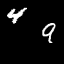
\includegraphics[width=0.4\textwidth]{3.png}
    \caption{DOUBLE-MNIST sample}
    \label{fig:double-mnist-sample}
\end{figure}

We ran our program on 3 different CNN multi-label DOUBLE-MNIST classifiers.
While the three of them solve the same classification problem, they differ in their training process:

\begin{itemize}
    \item Network with no defense - This network is trained regularly on the original DOUBLE-MNIST training dataset, without additional processing done to the training dataset.
    In Figure~\ref{fig:No defense} we present results of our program ran on this classifier and a single image, as a heatmap representing the epsilons per each layer.
    \begin{figure}
         \centering
         \begin{subfigure}[b]{0.4\textwidth}
             \centering
             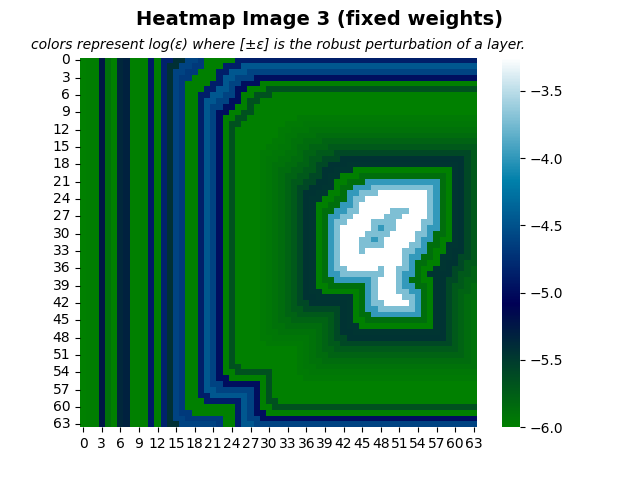
\includegraphics[width=\textwidth]{no_defense_fixed_weights.png}
             \caption{fixed weights}
             \label{sub-fig:No defense FW}
         \end{subfigure}
         \hfill
         \begin{subfigure}[b]{0.4\textwidth}
             \centering
             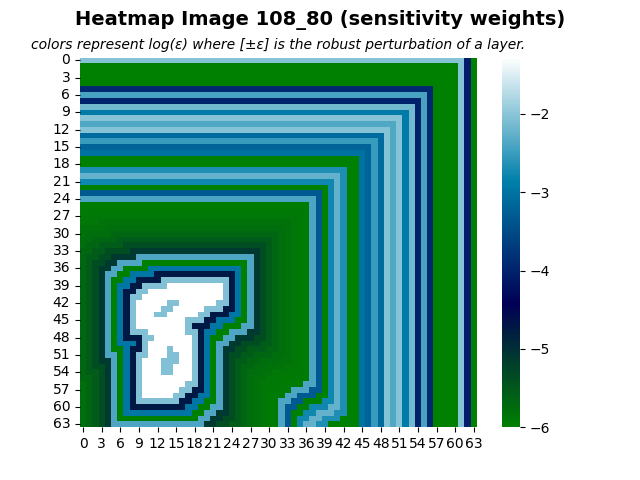
\includegraphics[width=\textwidth]{no_defense_sensitivity_weights.png}
             \caption{sensitivity weights}
             \label{sub-fig:No defense SW}
         \end{subfigure}
         \caption{No Defense}
         \label{fig:No defense}
     \end{figure}
    \item Network with $L_0$ defense - This network is trained with $L_0$ defense.
    To achieve this kind of defense, we add data-augmentation to the process of training;
    Before forwarding a training sample to the network, we add random noise to the image.
    Specifically, we randomly choose a rectangular section in the image and zero all its pixels (color them black).
    In Figure~\ref{fig:L0 defense} we present results of our program ran on this classifier and a single image, as a heatmap representing the epsilons per each layer.
    \begin{figure}
         \centering
         \begin{subfigure}[b]{0.4\textwidth}
             \centering
             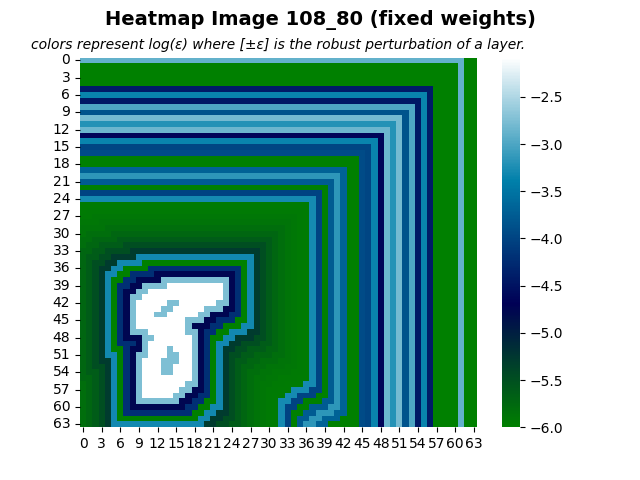
\includegraphics[width=\textwidth]{l0_defense_fixed_weights.png}
             \caption{fixed weights}
             \label{sub-fig:L0 defense FW}
         \end{subfigure}
         \hfill
         \begin{subfigure}[b]{0.4\textwidth}
             \centering
             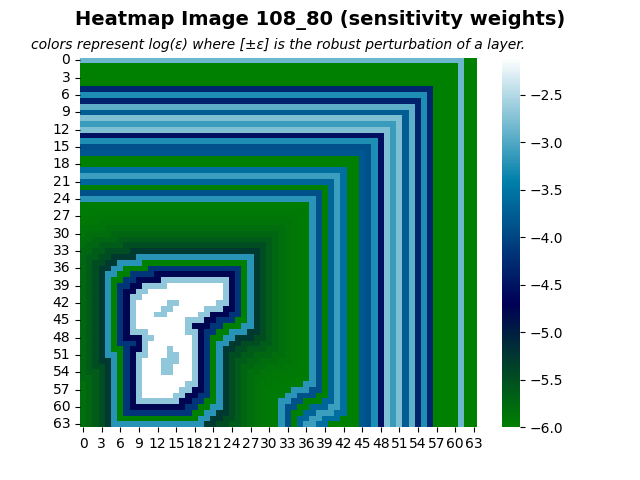
\includegraphics[width=\textwidth]{l0_defense_sensitivity_weights.png}
             \caption{sensitivity weights}
             \label{sub-fig:L0 defense SW}
         \end{subfigure}
         \caption{$L_0$ Defense}
         \label{fig:L0 defense}
    \end{figure}
    \item Network with $L_{\infty}$ defense - This network is trained with $L_{\infty}$ defense.
    To achieve this kind of defense, we also use data-augmentation, but this time we use PGD (Projected Gradient Descent)~\cite{PGD}.
    This also involves training the model with adversarial examples, but unlike the $L_0$ defense, the added perturbations can be anywhere in the input.
    The PGD generated adversarial examples are achieved by trying to increase the model's loss function as much as possible.
    Therefore, training the model with such adversarial examples should make the network more robust.
\end{itemize}